\section{Следящий регулятор}
Рассмотрим систему 
\begin{equation}
    \hat{x} = Ax + Bu, \quad x(0) = \begin{bmatrix}1 & 1 & 1\end{bmatrix}^T
\end{equation}
с генератором внешнего возмущения 
\begin{equation}
    \dot{w}_g = \Gamma w_g, \quad w_g(0) = \begin{bmatrix}1 & 1 & 1 & 1\end{bmatrix}^T
\end{equation}
и виртуальным выходом
\begin{equation}
    z = C_z x + D_z w_g 
\end{equation}
где 
\begin{equation}
    \begin{array}{cc}
        \begin{array}{cc}
            A = \begin{bmatrix}
                8 & 1 & 11 \\ 
                4 & 0 & 4 \\ 
                -4 & -3 & -7 \\ 
            \end{bmatrix}, & 
            B = \begin{bmatrix} -1 \\ -3 \\ 3 \end{bmatrix},
        \end{array} \\ 
        \begin{array}{ccc}
        C_z = \begin{bmatrix} -2 \\ -3 \\ -1 \end{bmatrix}^T, & 
        \Gamma = \begin{bmatrix}
            -40 & 16 & 9 & 7 \\ 
            -64 & 25 & 14 & 12 \\
            -26 & 11 & 7 & 3 \\ 
            -48 & 18 & 14 & 8 \\ 
        \end{bmatrix} & 
        D_z = \begin{bmatrix}8 \\ -8 \\ 12 \\ -3\end{bmatrix}^T
        \end{array}
    \end{array}
\end{equation}

Схема моделирования этой системы представлена на рисунке \ref{fig:scheme2}.
\begin{figure}[ht!]
    \centering
    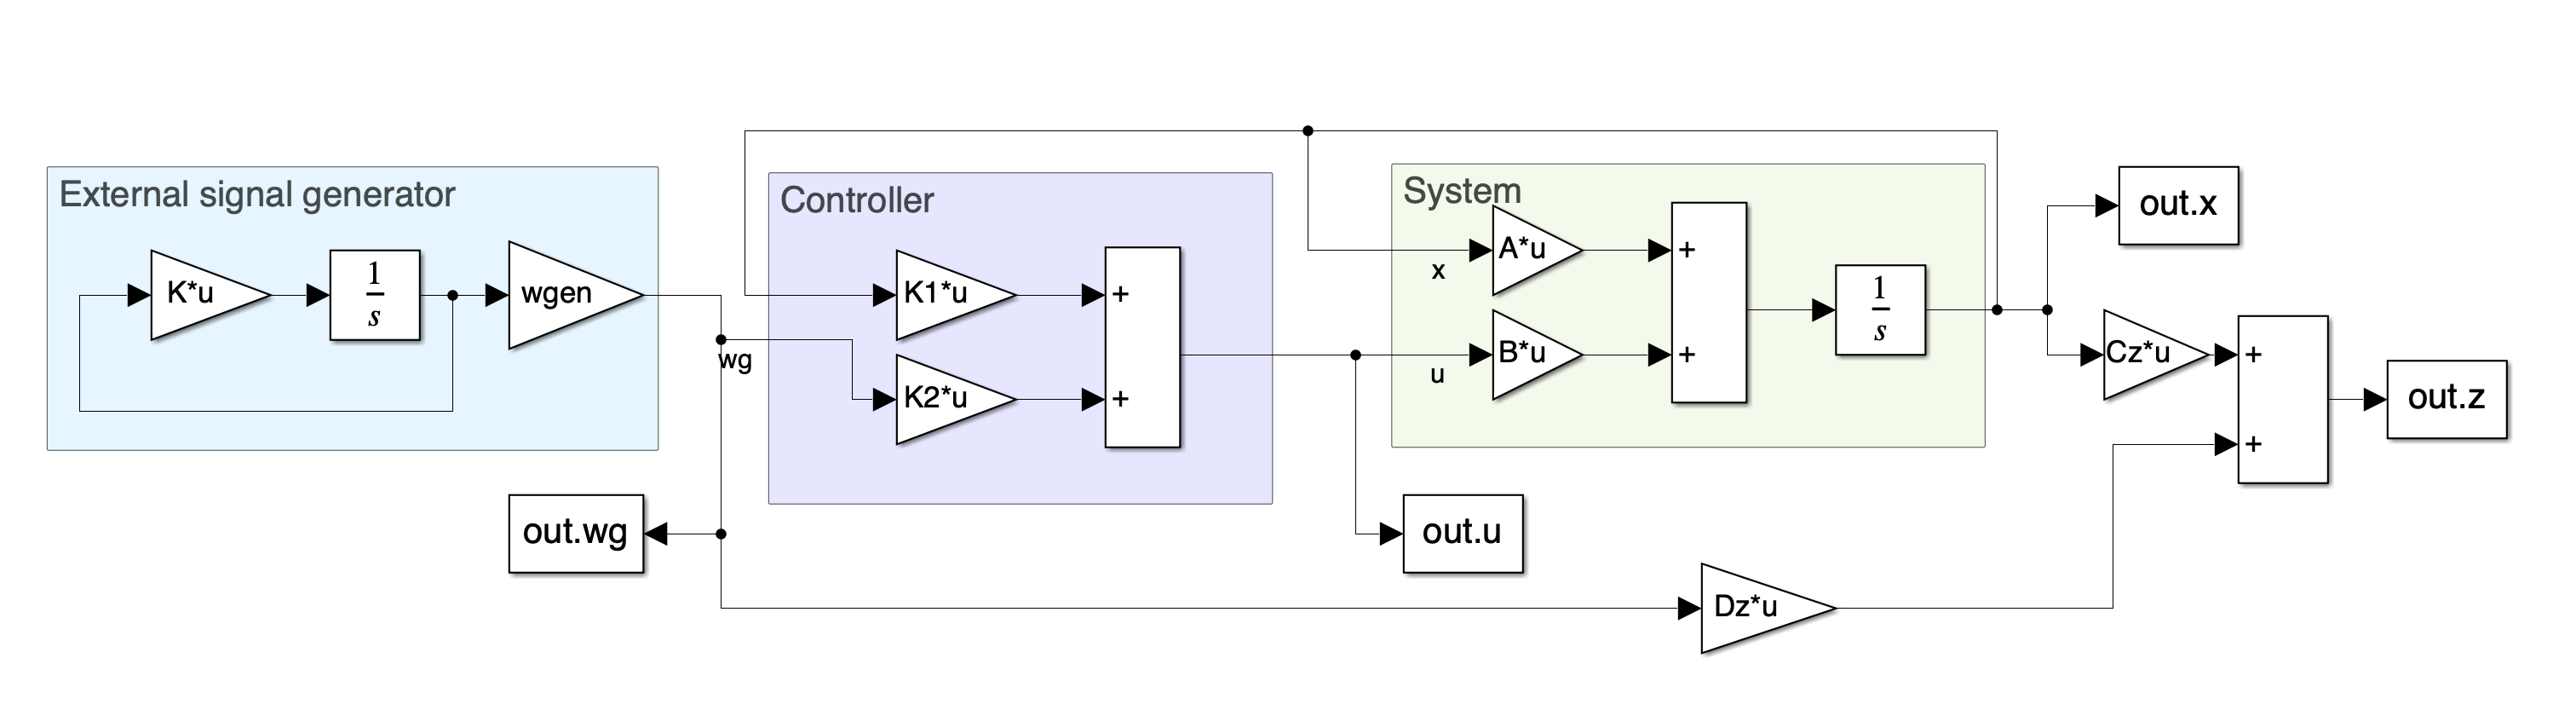
\includegraphics[width=\textwidth]{media/scheme2.png}
    \caption{Схема моделирования системы с следящим регулятором}
    \label{fig:scheme2}
\end{figure}
\FloatBarrier
\subsection{Анализ внешнего возмущения}
Согласно результатам, полученным ранее, входное воздействие представляет собой 
гармонический сигнал, состоящий из двух частот. График входного воздействия
представлен на рисунке \ref{fig:wf}.
Проведем моделирование разомкнутой системы ($u = 0$). Результаты моделирования
представлены на рисунке \ref{fig:task2_open_x} (график состояния системы) и
\ref{fig:task2_open_z} (график виртуального выхода системы).
\begin{figure}[ht!]
    \centering
    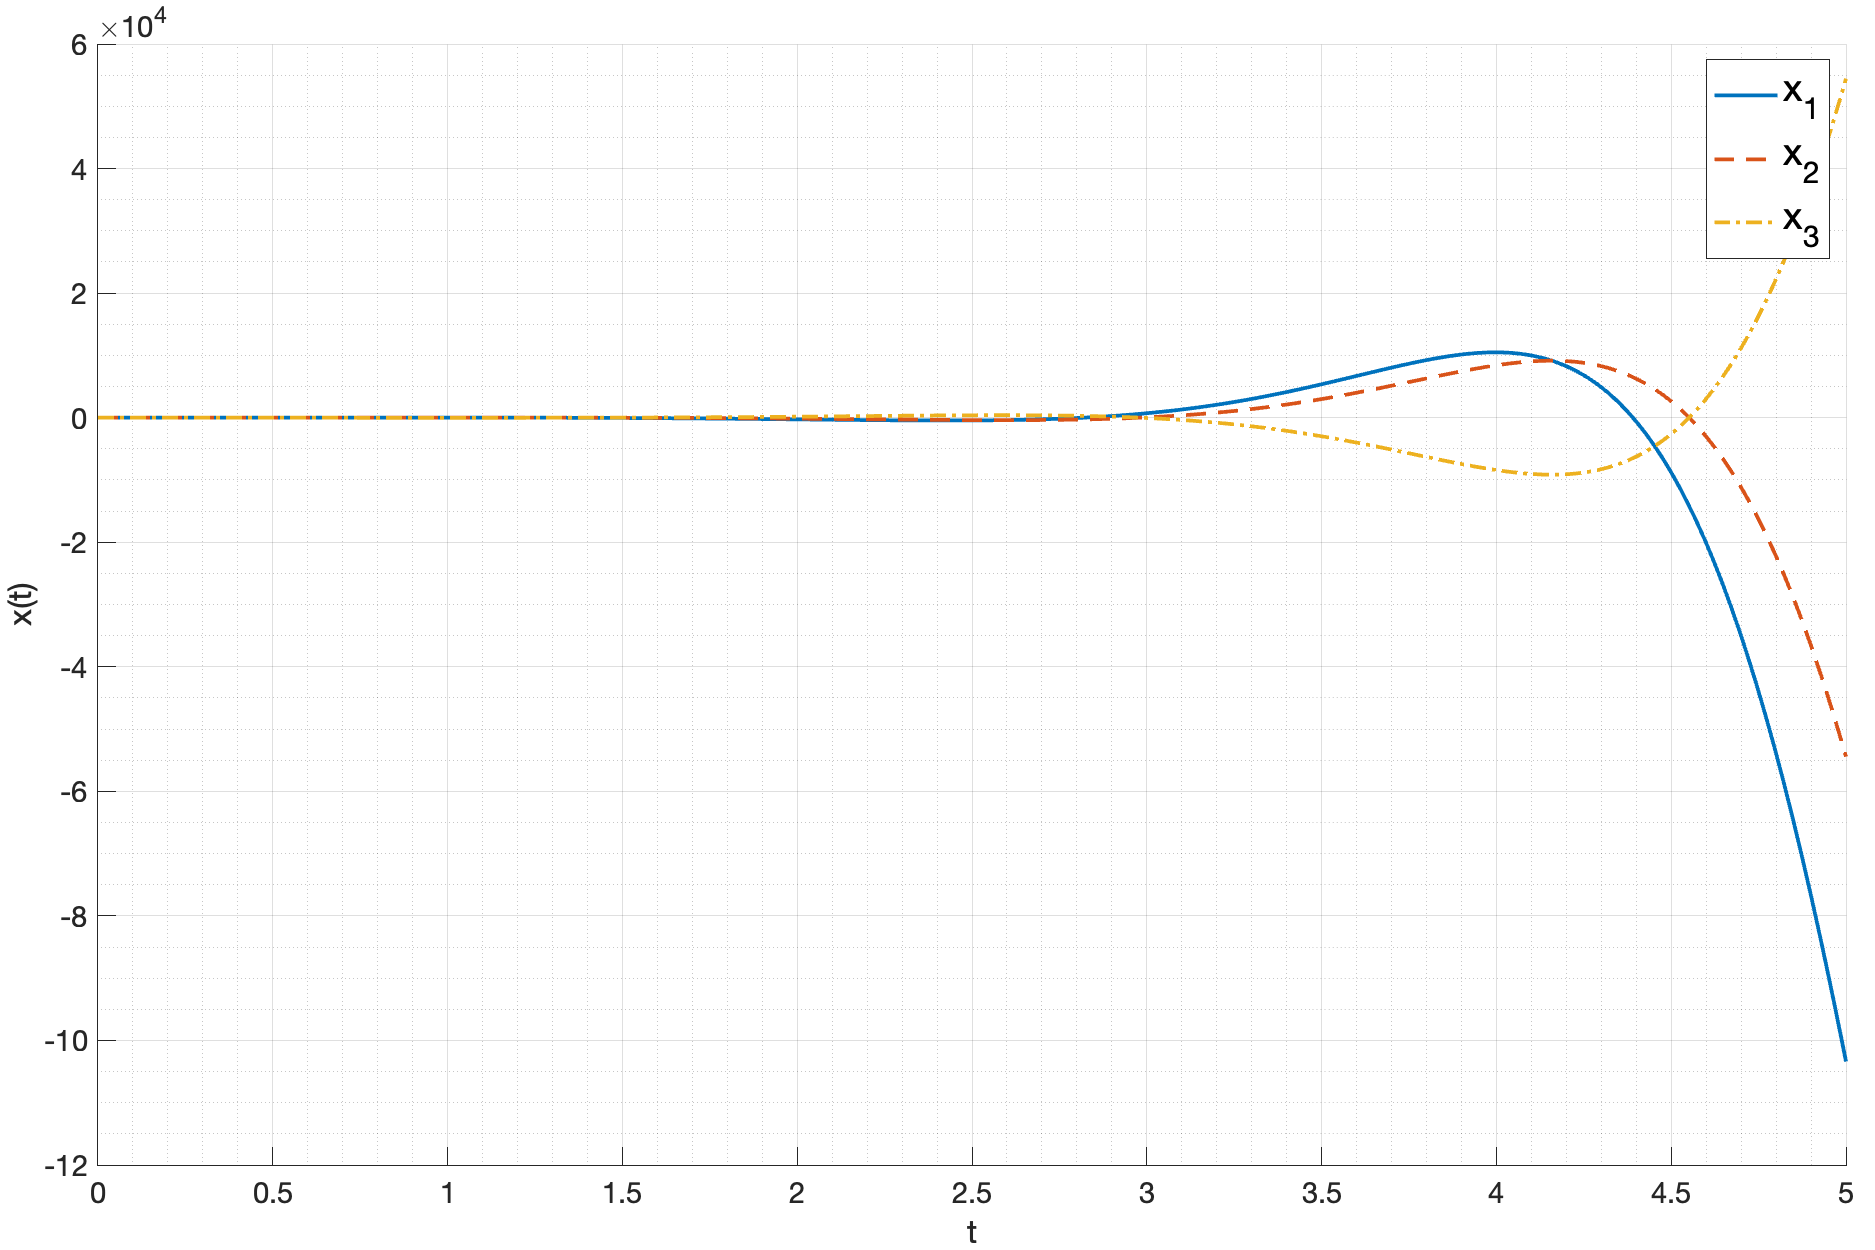
\includegraphics[width=\textwidth]{media/plots/task2_open_x.png}
    \caption{График состояния системы}
    \label{fig:task2_open_x}
\end{figure}
\begin{figure}[ht!]
    \centering
    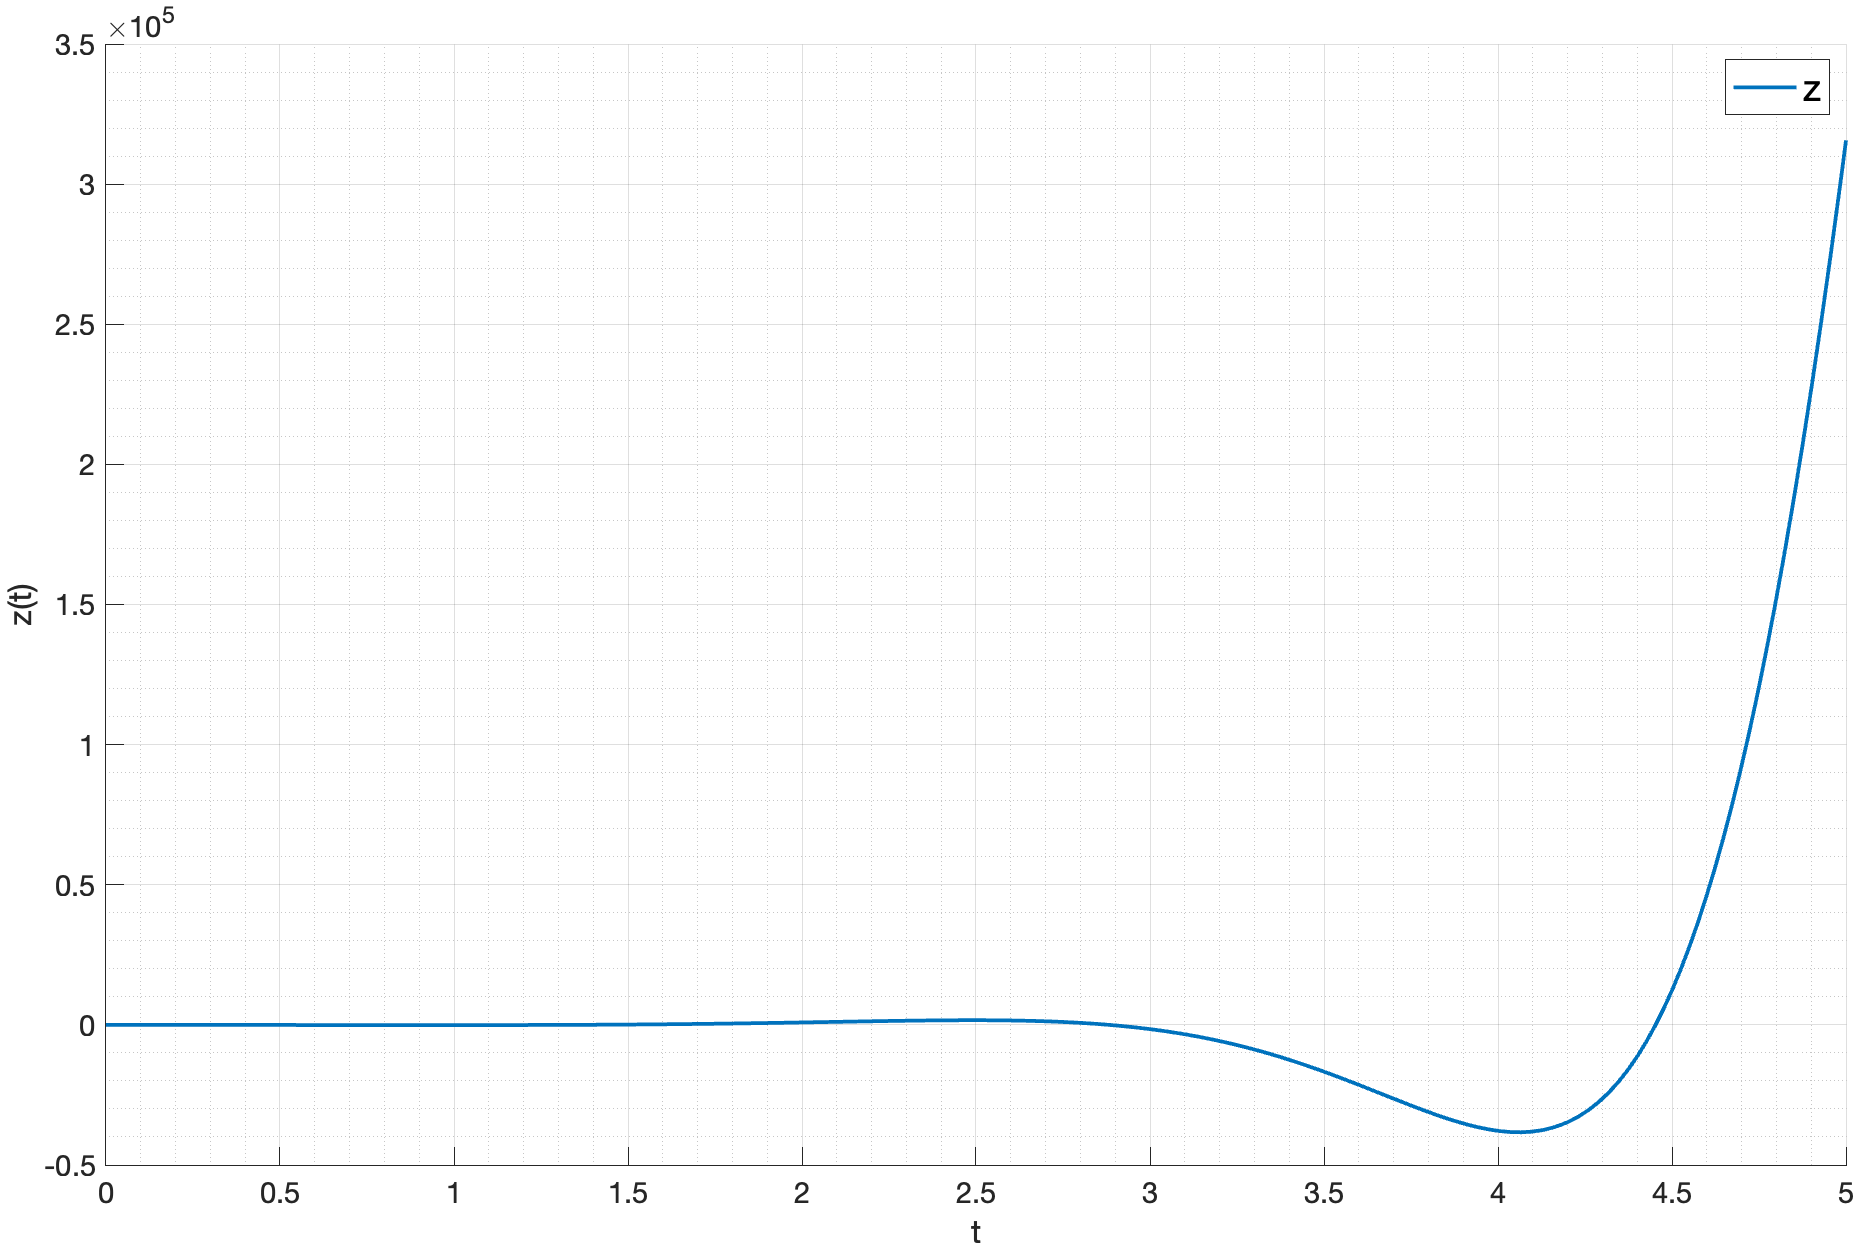
\includegraphics[width=\textwidth]{media/plots/task2_open_z.png}
    \caption{График виртуального выхода системы}
    \label{fig:task2_open_z}
\end{figure}
Видно, что система является неустойчивой. Состояние системы не сходится к нулю 
из-за неустойчивых собственных значений матрицы $A$. Виртуальный выход системы 
также не сходится к нулю, при этом это еще обусловлено и тем, что 
входной воздействие, которое является его частью не сходится к нулю. 
\FloatBarrier
\subsection{Синтез регулятора}
Как и в случае компенсирующего регулятора, синтез следящего регулятора 
будет состоять из двух этапов: синтез feedback компоненты и синтез feedforward компоненты. 

\subsubsection{Feedback компонента}
Синтез feedback компоненты будет идентичен такому же синтезу для
компенсирующего регулятора. Возьмем результаты из предыдущего пункта (\ref{eq:K1}). 
\begin{equation}
    K_1 = \begin{bmatrix}
        -4.57  & 0.29  & -4.57 \\ 
    \end{bmatrix}
\end{equation}
Промоделируем систему с полученным регулятором. Результаты моделирования 
представлены на рисунке \ref{fig:task2_K1_x} (график состояния системы) и
\ref{fig:task2_K1_z} (график виртуального выхода системы).
\begin{figure}[ht!]
    \centering
    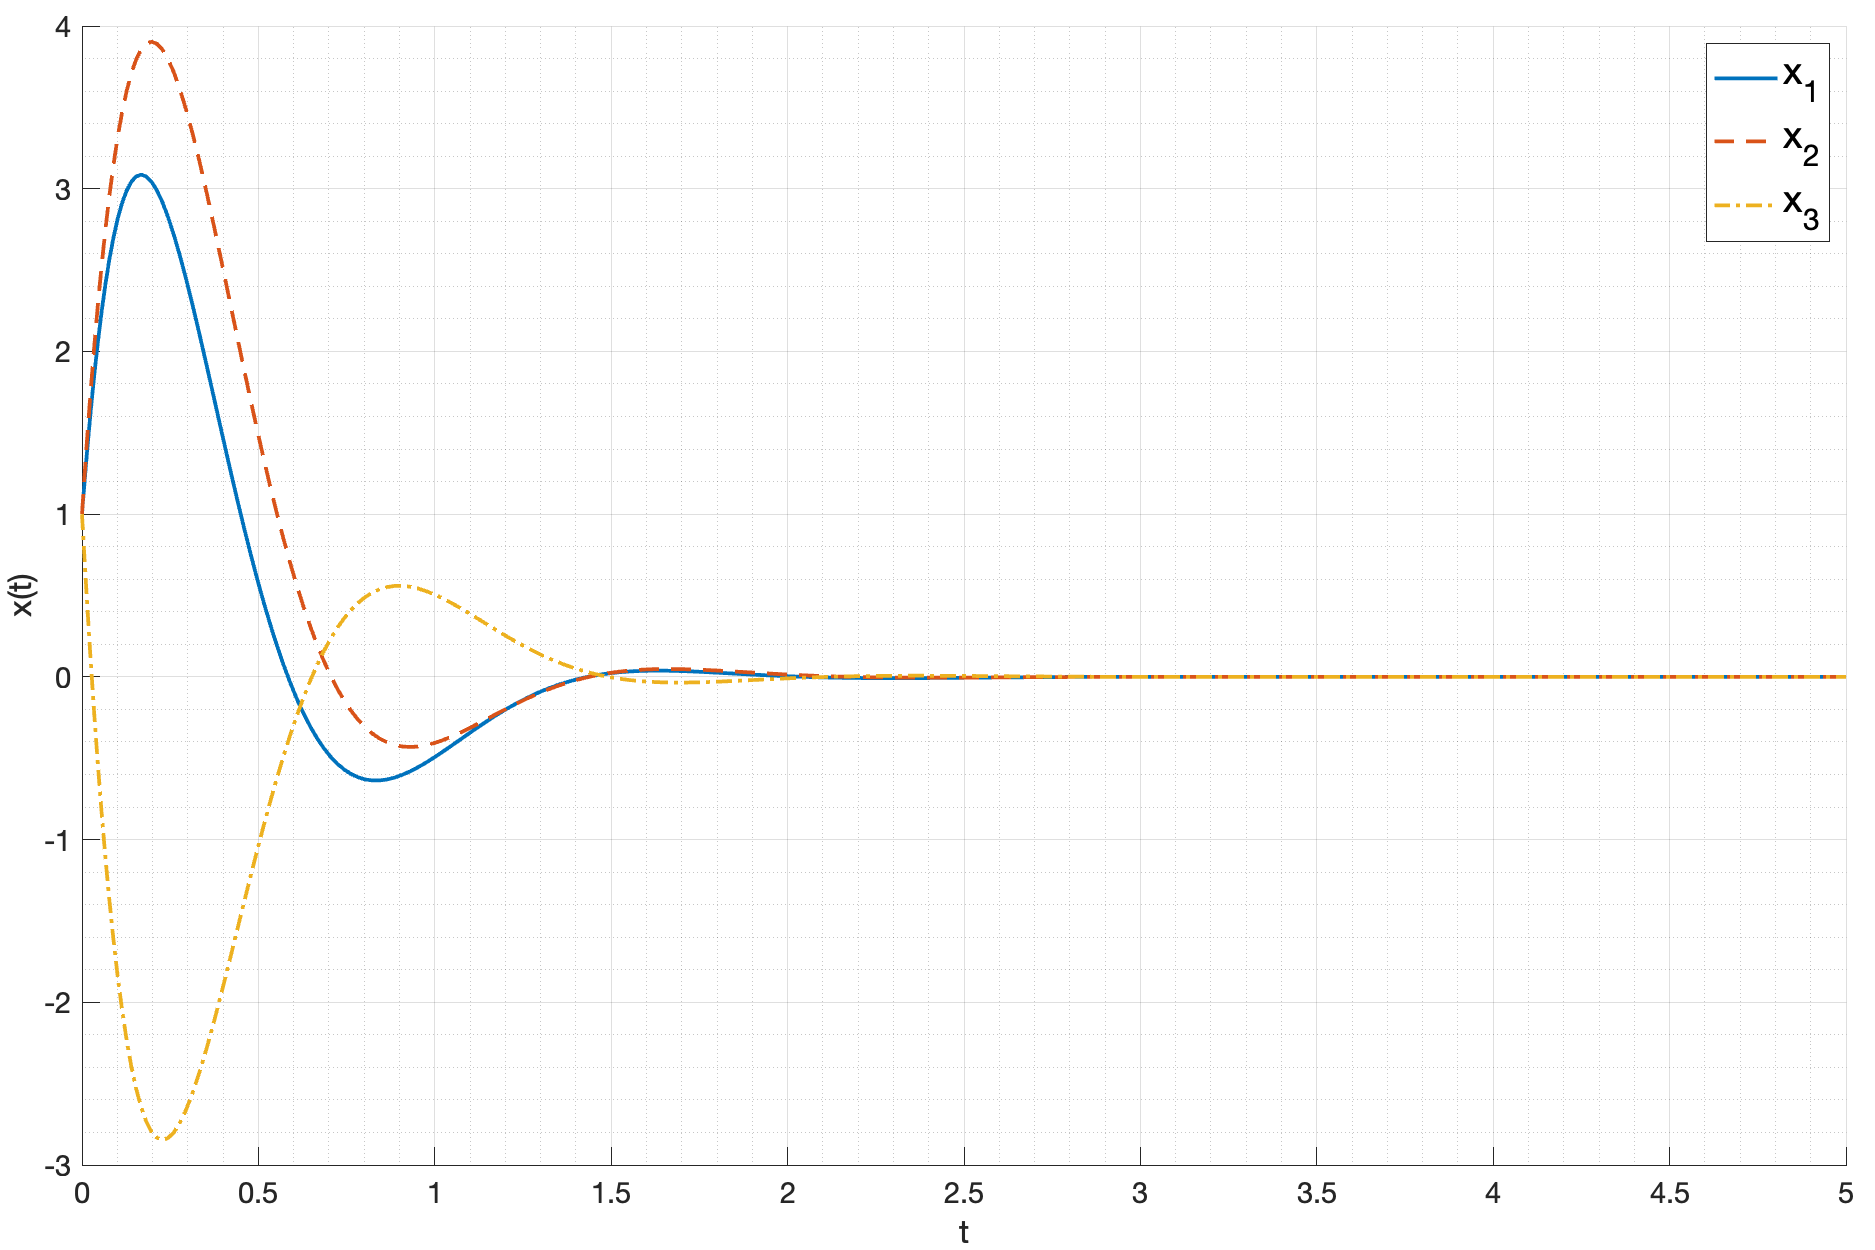
\includegraphics[width=\textwidth]{media/plots/task2_K1_x.png}
    \caption{График состояния системы с регулятором $K_1$}
    \label{fig:task2_K1_x}
\end{figure}
\begin{figure}[ht!]
    \centering
    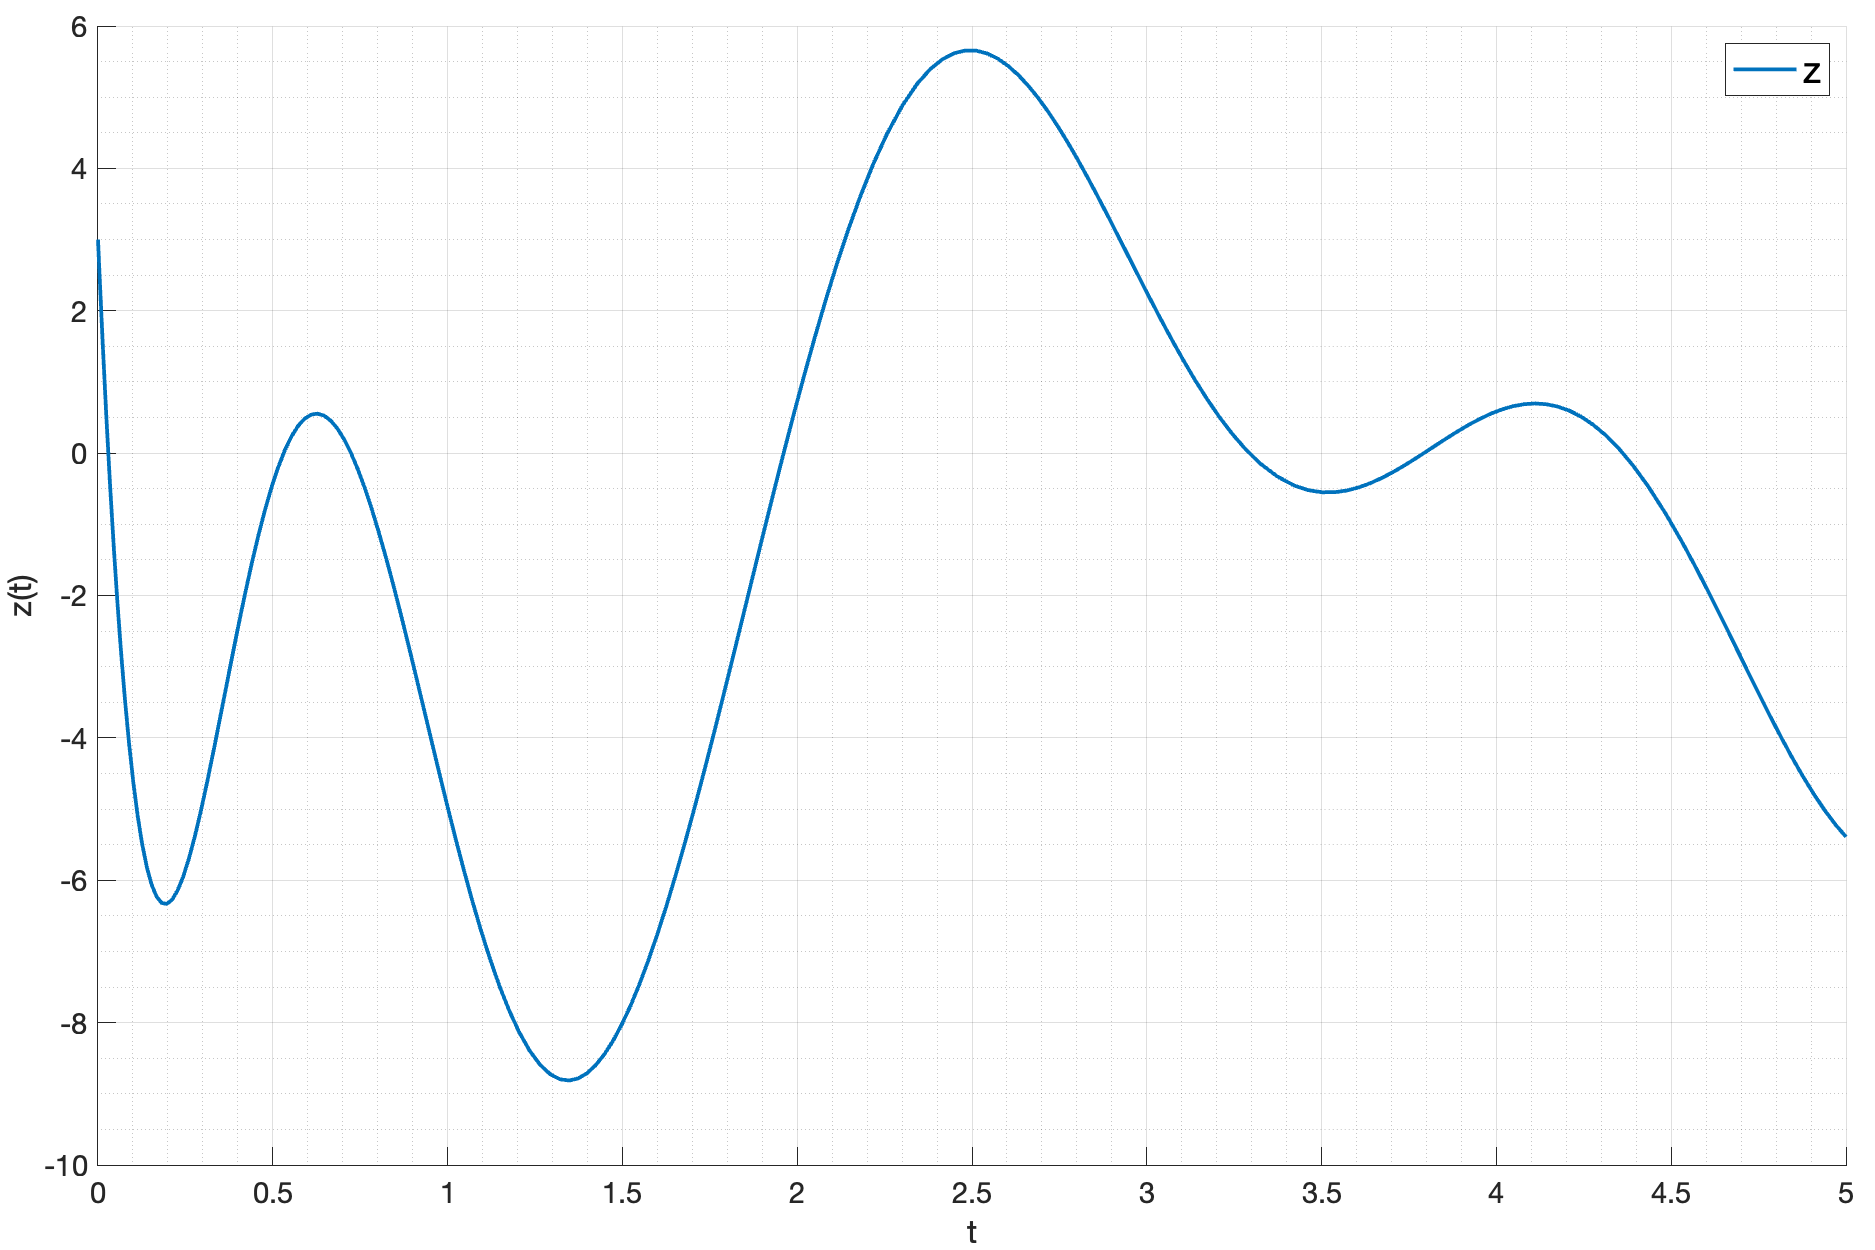
\includegraphics[width=\textwidth]{media/plots/task2_K1_z.png}
    \caption{График виртуального выхода системы с регулятором $K_1$}
    \label{fig:task2_K1_z}
\end{figure}
Видно, что регулятор справляется с задачей стабилизации состояния системы, но 
целевой параметр (виртуальный выход) не стабилизируется. Это связано с тем, что в его составе 
есть входное воздействие, которое не стабилизируется. 

\FloatBarrier
\subsubsection{Feedforward компонента}
Для синтеза следящего регулятора воспользуемся уравнениями: 
\begin{equation}
    \begin{cases}
        P\Gamma - AP = BY\\ 
        C_z P + D_z = 0 \\ 
        K_2 = Y - K_1 P \\ 
    \end{cases}
\end{equation}
Условием существования такого регулятора является принадлежность собственных чисел 
внешнего воздействия правой комплексной полуплоскости и принадлежность корней 
системы, замкнутой регулятором, левой комплексной полуплоскости. Оба эти условия выполняются. 
Решим систему с помощью пакета \texttt{cvx} в MATLAB, в результате получаем:
\begin{equation}
    K_2 = \begin{bmatrix}
        3.23  & -0.90  & 2.40  & -2.74 \\ 
    \end{bmatrix}
\end{equation}
Промоделируем систему с управлением $u = K_1x + K_2w_g$. Результаты
моделирования представлены на рисунке \ref{fig:task2_full_x} (график состояния системы) и
\ref{fig:task2_full_z} (график виртуального выхода системы).
\begin{figure}[ht!]
    \centering
    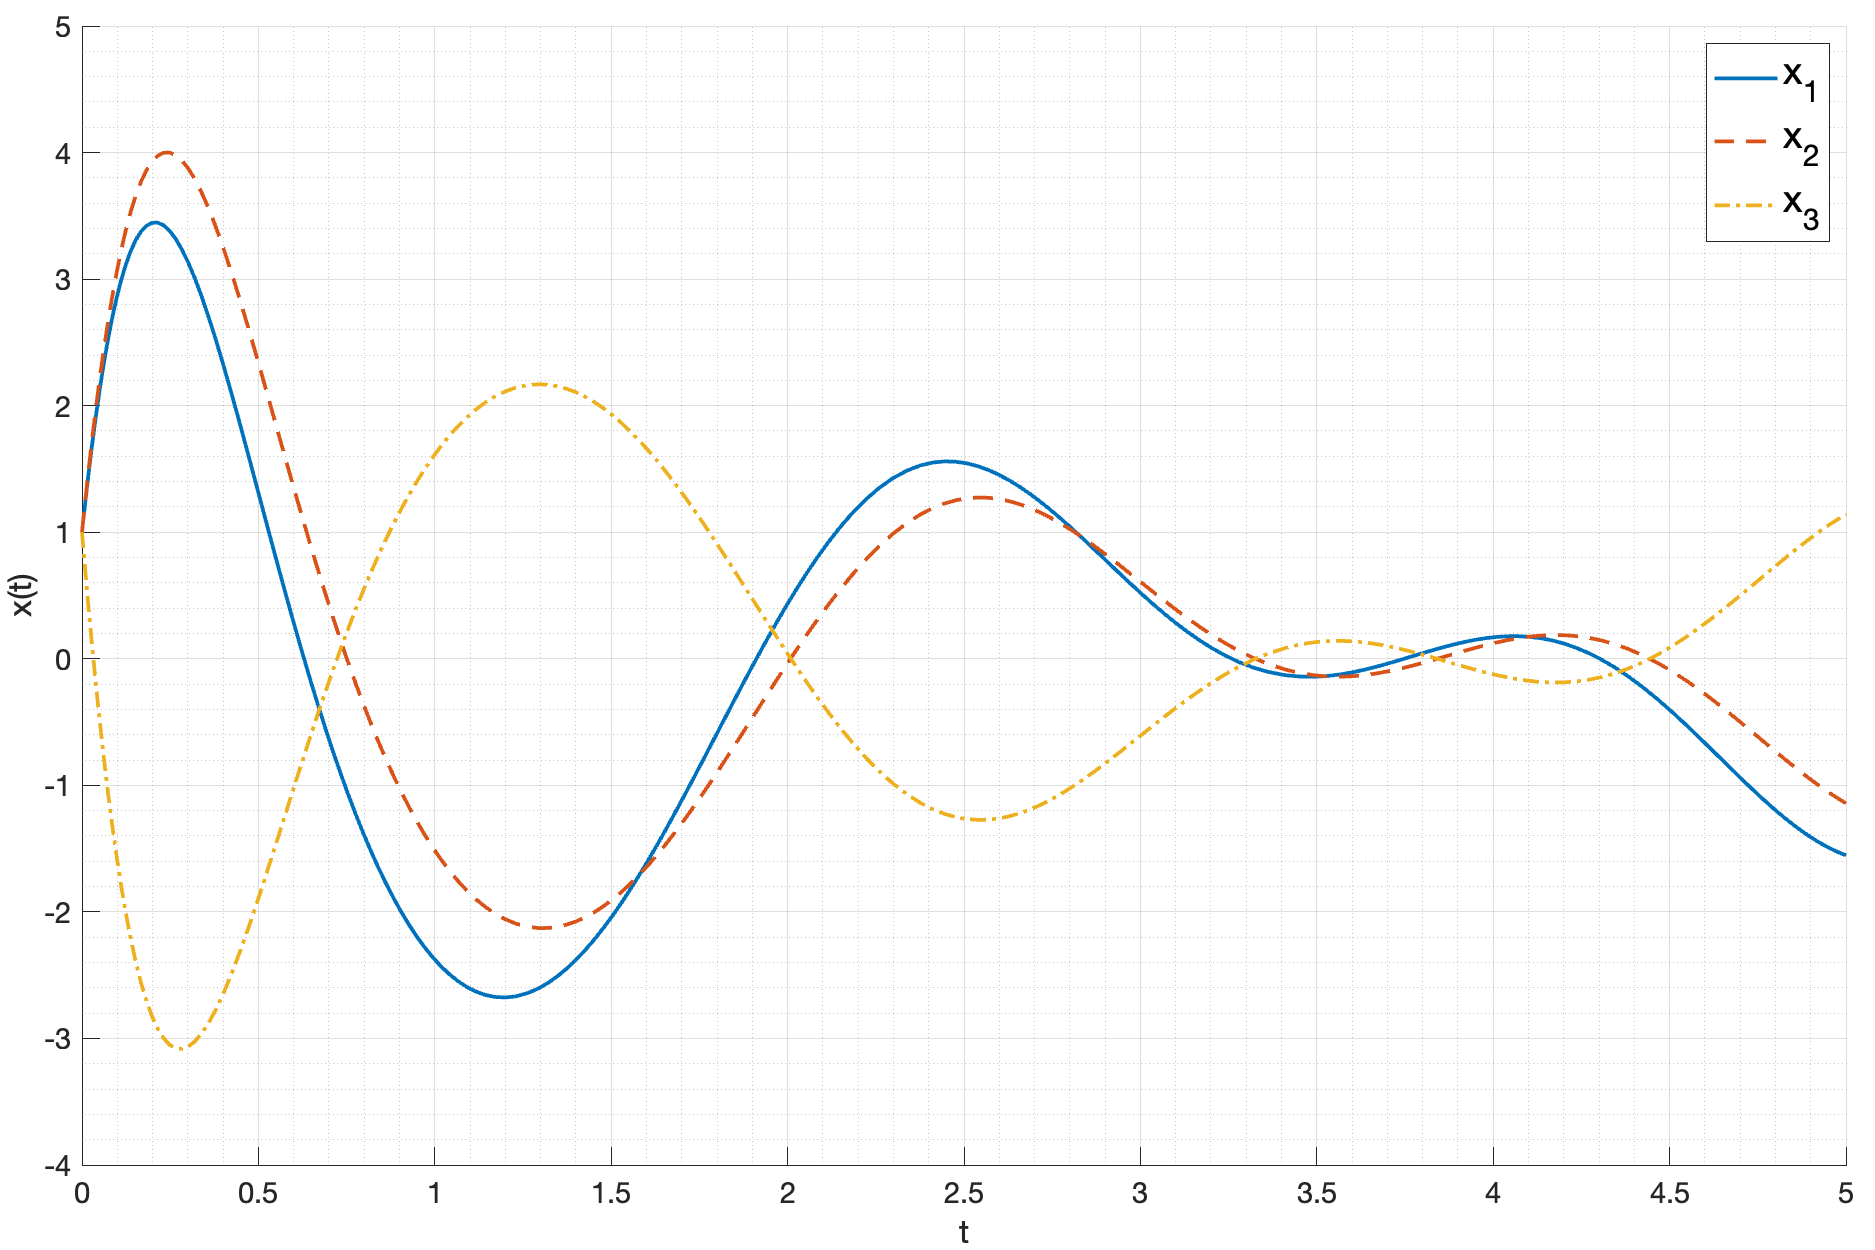
\includegraphics[width=\textwidth]{media/plots/task2_full_x.png}
    \caption{График состояния системы с регулятором $K_1 + K_2$}
    \label{fig:task2_full_x}
\end{figure}
\begin{figure}[ht!]
    \centering
    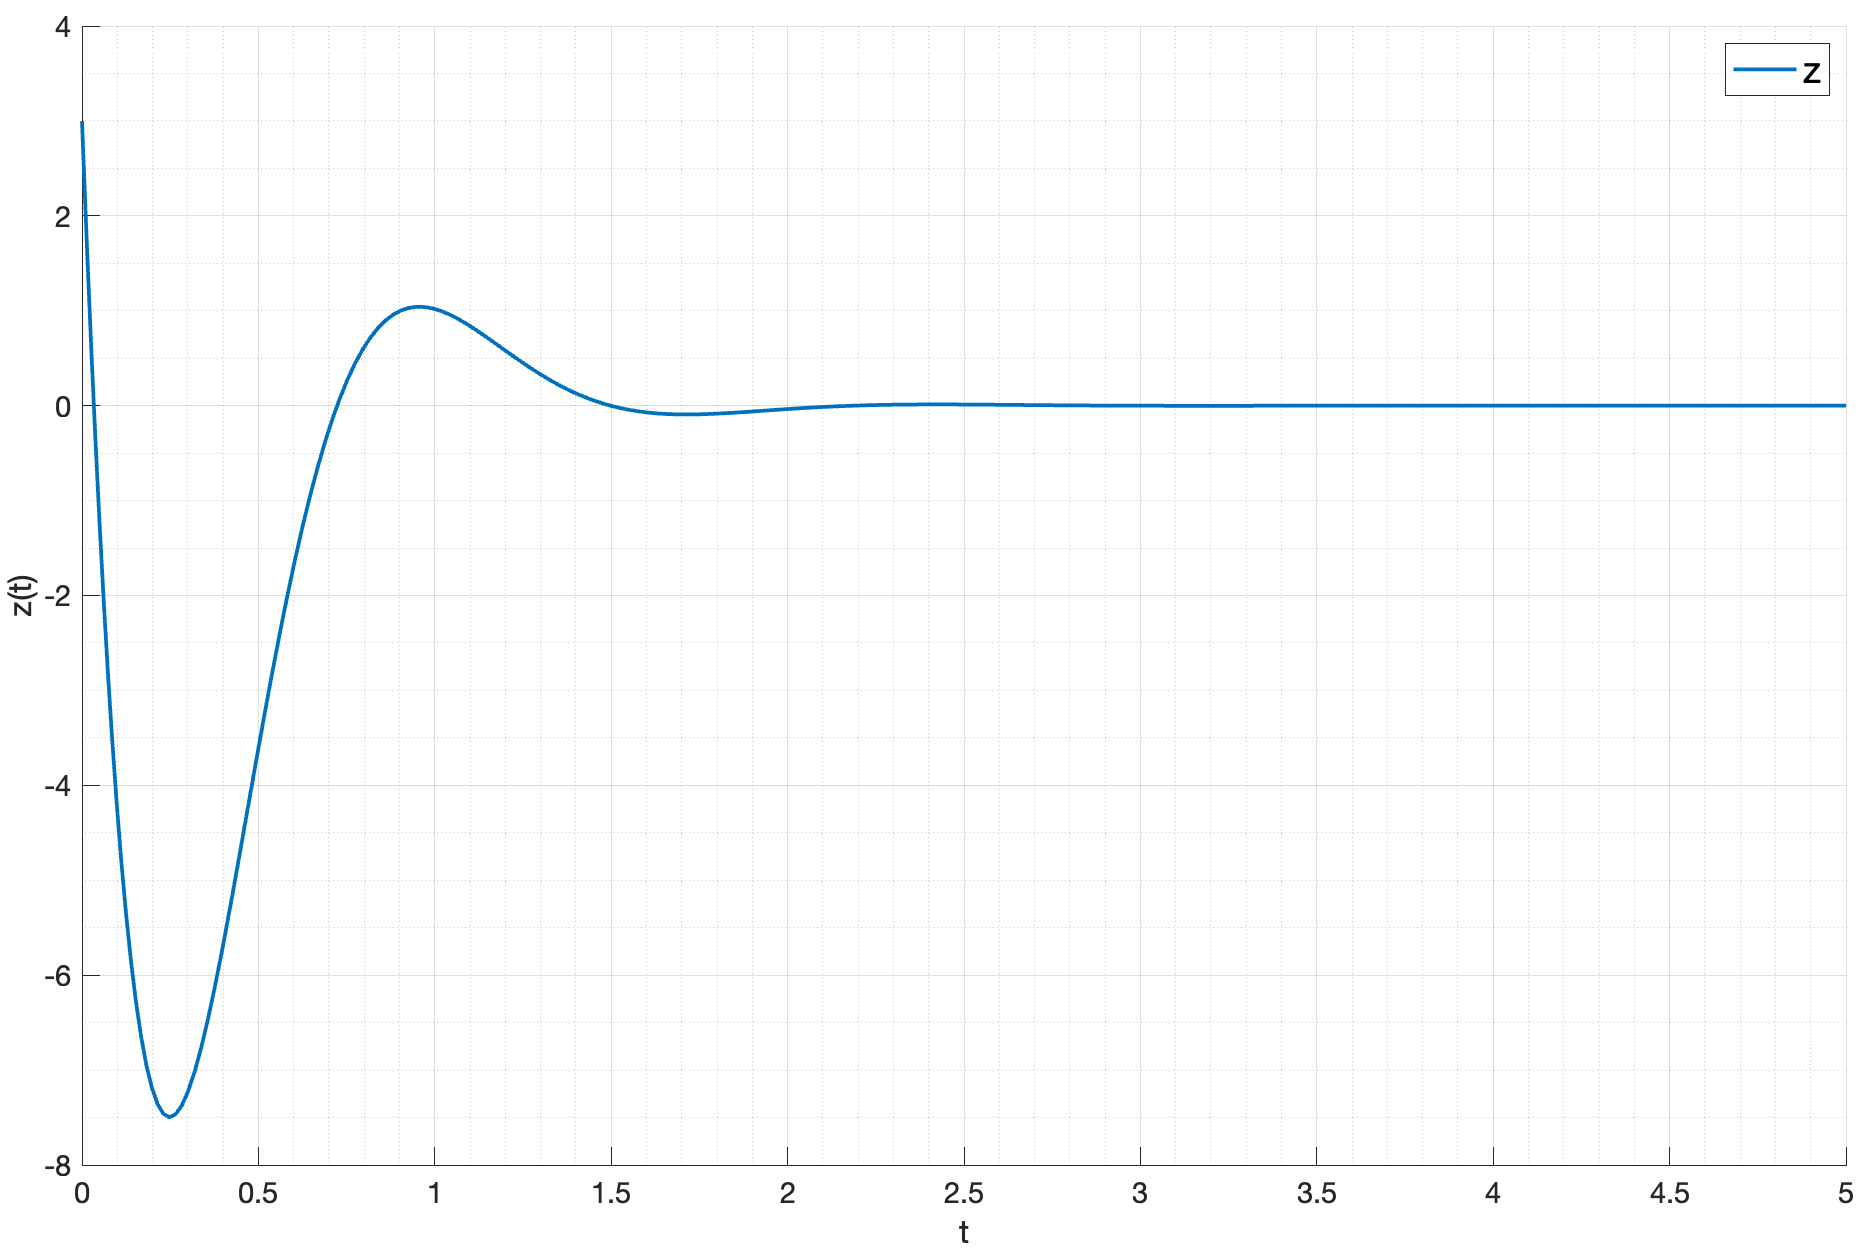
\includegraphics[width=\textwidth]{media/plots/task2_full_z.png}
    \caption{График виртуального выхода системы с регулятором $K_1 + K_2$}
    \label{fig:task2_full_z}
\end{figure}
Видно, что теперь виртуальный выход системы стабилизировался, что говорит о том, что 
регулятор справляется с задачей слежения за входным воздействием.

\FloatBarrier

Сравнительные графики приведены на рисунках \ref{fog:task2_cpm_u} (сравнение управления)
и \ref{fog:task2_cpm_z} (сравнение виртуального выхода).
\begin{figure}[ht!]
    \centering
    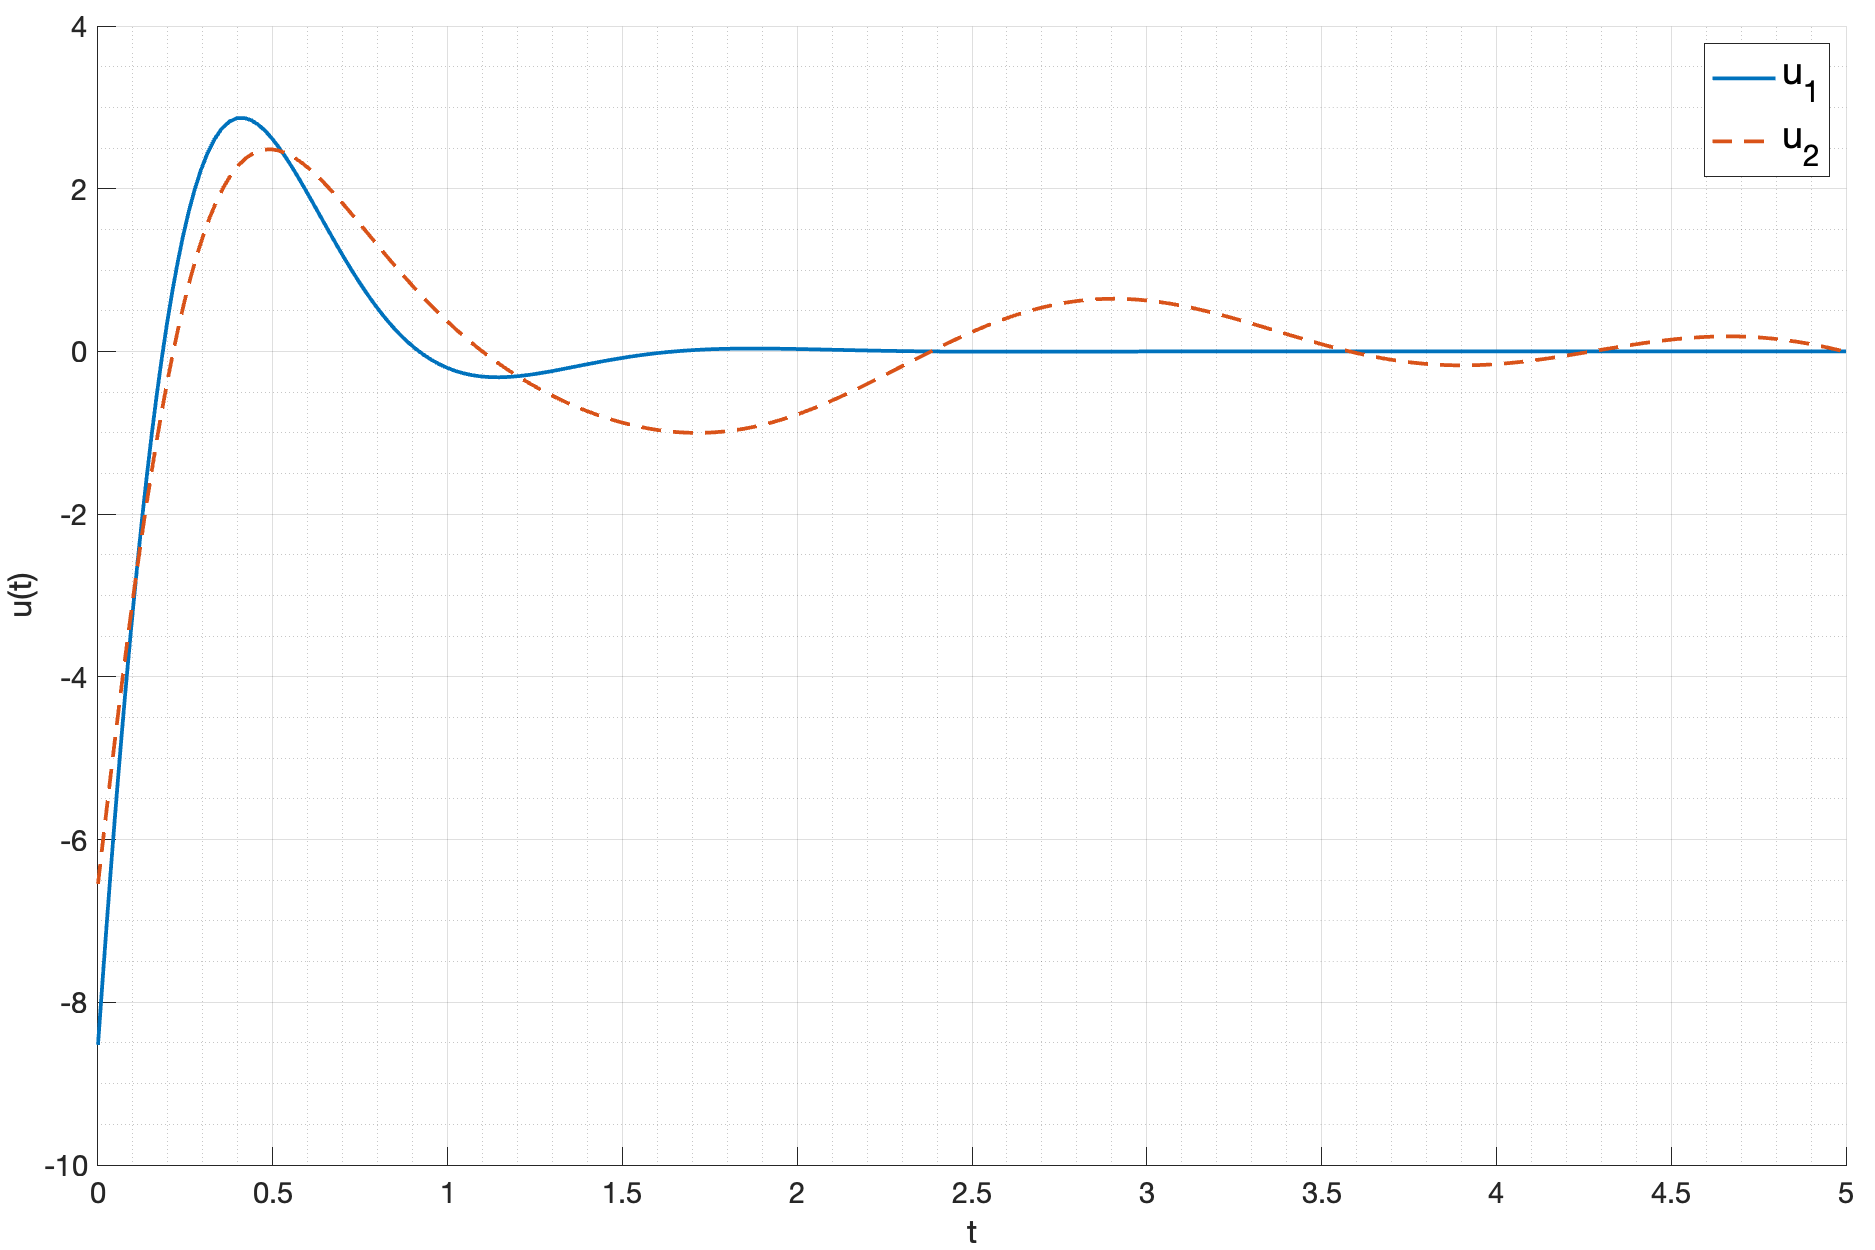
\includegraphics[width=\textwidth]{media/plots/task2_u_cmp.png}
    \caption{Сравнение управления}
    \label{fog:task2_cpm_u}
\end{figure}
\begin{figure}[ht!]
    \centering
    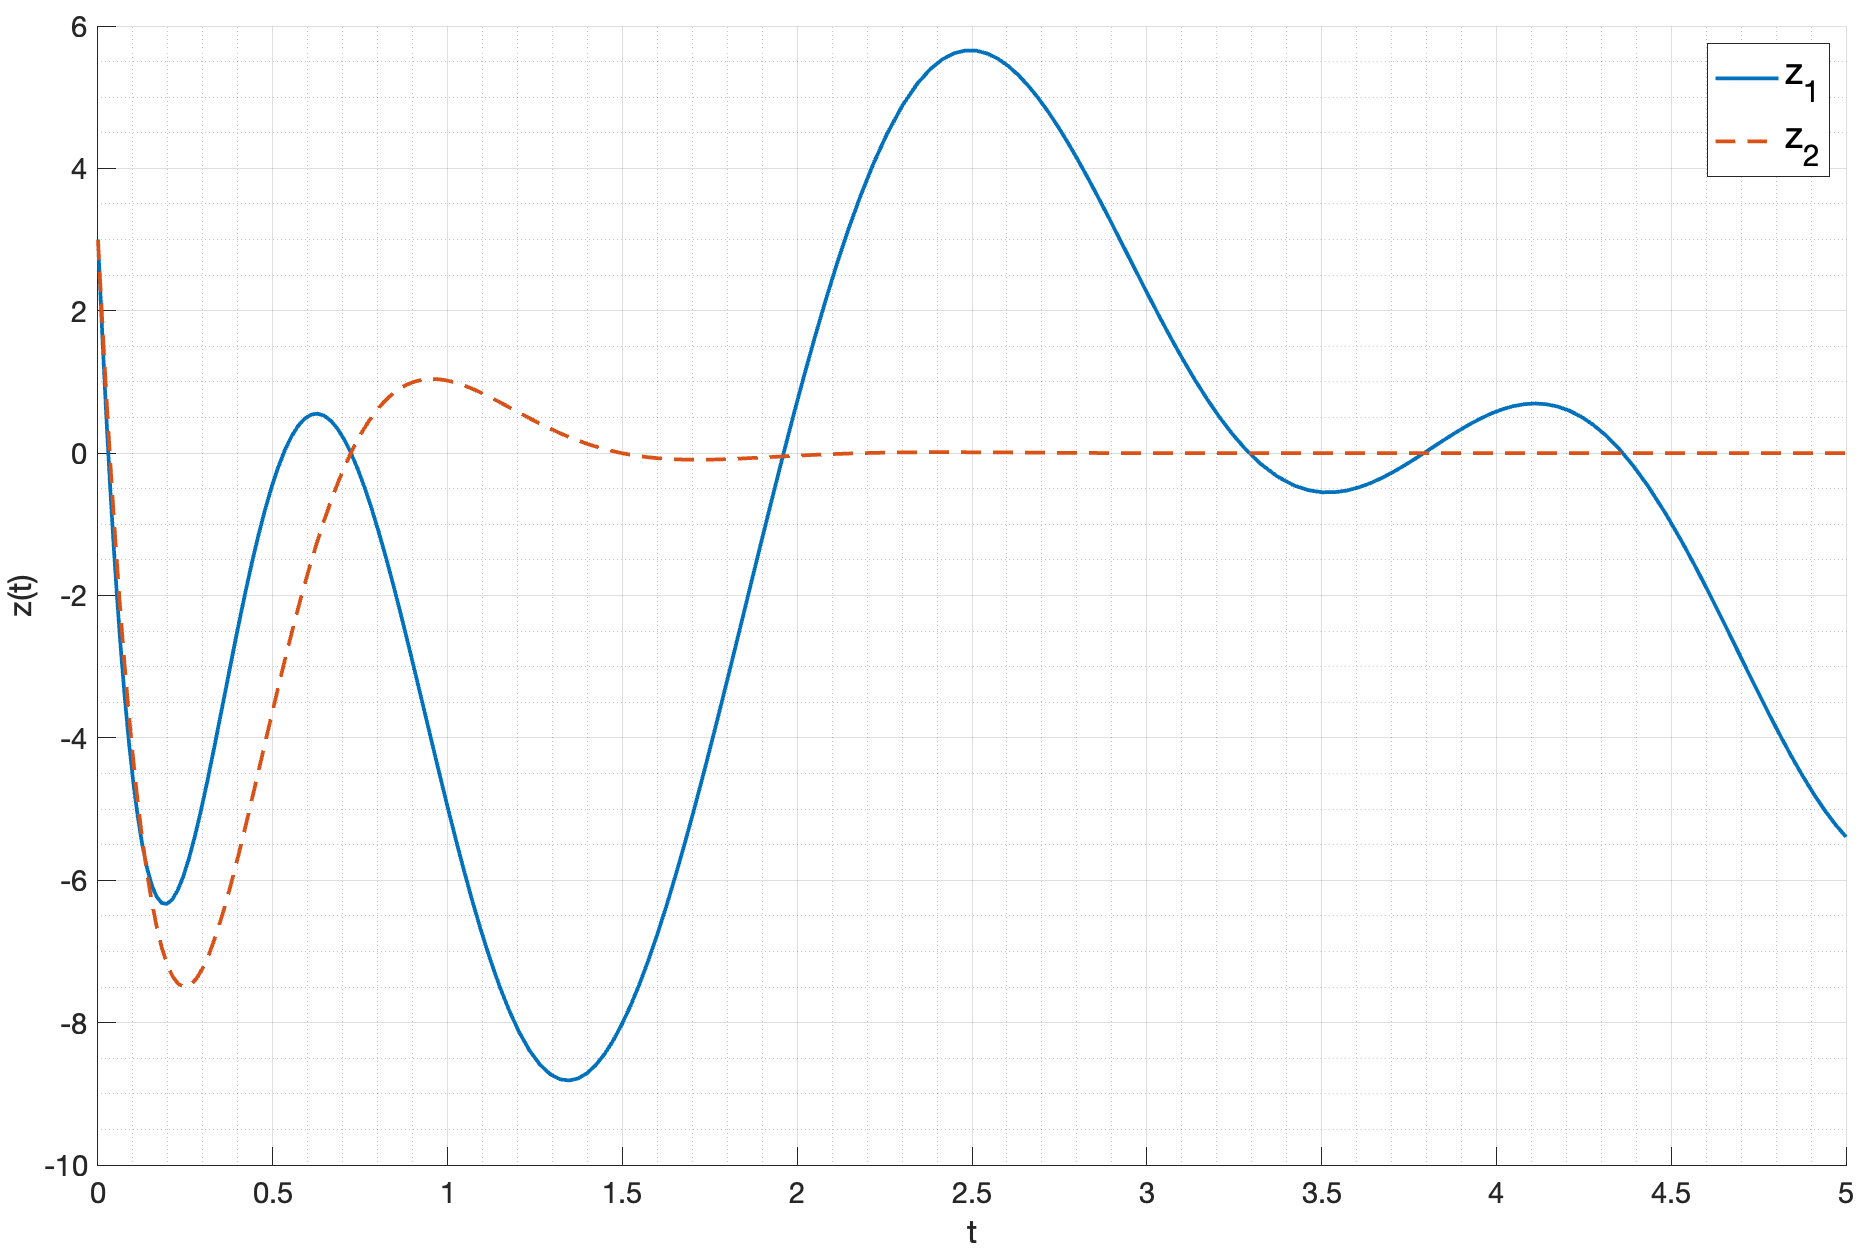
\includegraphics[width=\textwidth]{media/plots/task2_z_cmp.png}
    \caption{Сравнение виртуального выхода}
    \label{fog:task2_cpm_z}
\end{figure}
Где $u_1$ -- управление, формируемое регулятором $K_1$, $u_2$ -- управление, формируемое полным регулятором $K_1 + K_2$,
$z_1$ -- выход системы с регулятором $K_1$, $z_2$ -- выход системы с полным регулятором $K_1 + K_2$.

Видно, что управление, формируемое полным регулятором $K_1 + K_2$ не сходится к нулю, 
в отличие от управления, формируемого регулятором $K_1$. Это связано с тем, что 
полный регулятор $K_1 + K_2$ учитывает входное воздействие, которое не стабилизируется. 
Таким образом получается добиться целевой задачи -- виртуальный выход системы
сходится к нулю. 
\FloatBarrier

\subsection{Выводы}
В данном пункте был рассмотрен регулятор, способный следить за входным воздействием. 
Как и в прошлом случае, синтез регулятора состоял из двух этапов: синтез feedback компоненты, 
которая обеспечивает устойчивость системы, которая осталась неизменной в силу 
неизменности системы и синтез feedforward компоненты, которая обеспечивает 
стабилизацию виртуального выхода системы. 

